\documentclass{scrreprt}

\usepackage{aligned-overset}
\usepackage{amsmath}
\usepackage{amsthm}
\usepackage{amssymb}
\usepackage{bm}
\usepackage[shortlabels]{enumitem}
\usepackage{framed}
\usepackage{hyperref}
\usepackage[utf8]{inputenc}
\usepackage{multicol}
\usepackage{mathtools}
\usepackage{pdflscape}
\usepackage{physics}
\usepackage{polynom}
\usepackage{tabularx}
\usepackage[table]{xcolor}
\usepackage{titling}
\usepackage{fancyhdr}
\usepackage{xfrac}
\usepackage{pgfplots}

\pgfplotsset{compat = newest}
\usepgfplotslibrary{fillbetween}
\usetikzlibrary{calc}
\usetikzlibrary{patterns}
\usetikzlibrary{through}


\author{Karsten Lehmann \\ 4935758}
\date{WiSe 2024/25}
\title{Nachbereitungsaufgaben 8\\INF-B-110, Lineare Algebra}

\setlength{\headheight}{26pt}
\pagestyle{fancy}
\fancyhf{}
\lhead{\thetitle}
\rhead{\theauthor}
\lfoot{\thedate}
\rfoot{Seite \thepage}

\begin{document}
\paragraph{N 7.2}
Es seien $m_1 \quad m_2 \quad m_3 \quad m_4 \quad m_5 \quad m_6 \quad m_7$ die
Ziffern Ihrer Matrikelnummer.

Es seien $f \colon \mathbb{R}^2 \to \mathbb{R}^2$ und
$g \colon \mathbb{R}^2 \to \mathbb{R}^2$ lineare Abbildungen mit
\[
  f\qty(\begin{pmatrix} m_1 \\ m_7 \end{pmatrix})
  = \begin{pmatrix} 1 \\ 0 \end{pmatrix}, \quad
  f\qty(\begin{pmatrix} 0 \\ m_1 \end{pmatrix})
  = \begin{pmatrix} 0 \\ 1 \end{pmatrix}, \qquad
  g\qty(\begin{pmatrix} 1 \\ 0 \end{pmatrix})
  = \begin{pmatrix} m_3 \\ m_6 \end{pmatrix}, \quad
  g\qty(\begin{pmatrix} 0 \\ 1 \end{pmatrix})
  = \begin{pmatrix} m_4 \\ m_5 \end{pmatrix}
\]
\begin{enumerate}[(a)]
\item Warum sind $f$ und $g$ dadurch eindeutig festgelegt?
  Ist $h \coloneqq g \circ f$ ebenfalls eine lineare Abbildung?

  \begin{small}
    Hinweis: Begründen Sie mit Hilfe geeigneter Aussagen aus der
    Lehrveranstaltung.
  \end{small}

  \subparagraph{Lsg.} Die einzelnen Ziffern der Matrikelnummer sind

  \begin{tabular}{|c|c|c|c|c|c|c|}
    \hline
    4 & 9 & 3 & 5 & 7 & 5 & 8 \\
    \hline
    $m_1$ & $m_2$ & $m_3$ & $m_4$ & $m_5$ & $m_6$ & $m_7$ \\
    \hline
  \end{tabular}

  und somit
  \[
    f\qty(\begin{pmatrix} 4 \\ 8 \end{pmatrix})
    = \begin{pmatrix} 1 \\ 0 \end{pmatrix}, \quad
    f\qty(\begin{pmatrix} 0 \\ 4 \end{pmatrix})
    = \begin{pmatrix} 0 \\ 1 \end{pmatrix}, \qquad
    g\qty(\begin{pmatrix} 1 \\ 0 \end{pmatrix})
    = \begin{pmatrix} 3 \\ 5 \end{pmatrix}, \quad
    g\qty(\begin{pmatrix} 0 \\ 1 \end{pmatrix})
    = \begin{pmatrix} 5 \\ 7 \end{pmatrix}
  \]
  Nun sind $\begin{pmatrix} 4 \\ 8 \end{pmatrix}$ und
  $\begin{pmatrix} 0 \\ 4 \end{pmatrix}$ offensichtlich linear unabhängig und
  bilden somit eine Basis von $\mathbb{R}^2$.
  Weiter ist $\qty(\qty\big(1, 0)^T, \qty\big(0, 1)^T)$ die Standardbasis von
  $\mathbb{R}^2$.

  Nun wurde in der Lehrveranstaltung bereits gezeigt, dass für jede Basis
  $B = \qty\big(b_1, b_2)$ und lineare Abbildung $f$ die Abbildung durch die
  Bilder der Basisvektoren bereits eindeutig bestimmt ist, da sich jedes
  $x \in \mathbb{R}^2$ als Linearkombination
  $x = \lambda \cdot b_1 + \mu \cdot b_2$ darstellen lässt und aus der Defintion
  einer linearen Funktion
  \[
    f\qty\big(\lambda \cdot b_1 + \mu \cdot b_2)
    = \lambda \cdot f\qty\big(b_1) + \mu \cdot f\qty\big(b_2)
  \]
  folgt.

  Nun wurde in Ü8.3 bereits gezeigt, dass auch die Komposition linearer Abbildungen
  wieder eine lineare Abbildung ist.
  Somit ist auch $h$ wieder linear.

\item Bestimmen Sie die Darstellungsmatrizen von $f$, von $g$ und von $h$
  bezüglich der Standarbasis von $\mathbb{R}^2$.

  \subparagraph{Lsg.} Es ist $B = \qty(\qty\big(1, 0)^T, \qty\big(0, 1)^T)$ die
  Standardbasis in $\mathbb{R}^2$.

  Nun sind
  \[
    f\qty(\begin{pmatrix} 1 \\ 0 \end{pmatrix})
    = f\qty(\frac{1}{4}\begin{pmatrix} 4 \\ 8 \end{pmatrix} - \frac{2}{4}\begin{pmatrix} 0 \\ 4 \end{pmatrix})
    = \frac{1}{4}f\qty(\begin{pmatrix} 4 \\ 8 \end{pmatrix}) - \frac{2}{4}f\qty(\begin{pmatrix} 0 \\ 4 \end{pmatrix})
    = \frac{1}{4}\begin{pmatrix} 1 \\ 0 \end{pmatrix} - \frac{2}{4}\begin{pmatrix} 0 \\ 1 \end{pmatrix}
    = \begin{pmatrix} \frac{1}{4} \\ -\frac{1}{2} \end{pmatrix}
  \]
  \[
    f\qty(\begin{pmatrix} 0 \\ 1 \end{pmatrix})
    = f\qty(0 \cdot \begin{pmatrix} 4 \\ 8 \end{pmatrix} + \frac{1}{4}\begin{pmatrix} 0 \\ 4 \end{pmatrix})
    = 0 \cdot f\qty(\begin{pmatrix} 4 \\ 8 \end{pmatrix}) + \frac{1}{4}f\qty(\begin{pmatrix} 0 \\ 4 \end{pmatrix})
    = \frac{1}{4}\begin{pmatrix} 0 \\ 1 \end{pmatrix}
    = \begin{pmatrix} 0 \\ \frac{1}{4} \end{pmatrix}
  \]
  und somit $A_{B, B}\qty\big(f) = \begin{pmatrix}
    \frac{1}{4}  & 0           \\
    -\frac{1}{2} & \frac{1}{4} \\
  \end{pmatrix}$.
  Außerdem ist $A_{B, B}\qty\big(g) = \begin{pmatrix}
    3 & 5 \\
    5 & 7 \\
  \end{pmatrix}$.

  \newpage
  Weiter ist
  \begin{flalign*}
    h\qty(\begin{pmatrix} 1 \\ 0 \end{pmatrix})
    &= g\qty(f\qty(\begin{pmatrix} 1 \\ 0 \end{pmatrix}))
    = g\qty(f\qty(\frac{1}{4}\begin{pmatrix} 4 \\ 8 \end{pmatrix} - \frac{2}{4}\begin{pmatrix} 0 \\ 4 \end{pmatrix})) &\\
    &= g\qty(\frac{1}{4}f\qty(\begin{pmatrix} 4 \\ 8 \end{pmatrix}) - \frac{2}{4}f\qty(\begin{pmatrix} 0 \\ 4 \end{pmatrix}))
    = \frac{1}{4}g\qty(f\qty(\begin{pmatrix} 4 \\ 8 \end{pmatrix})) - \frac{2}{4}g\qty(f\qty(\begin{pmatrix} 0 \\ 4 \end{pmatrix})) \\
    &= \frac{1}{4}g\qty(\begin{pmatrix} 1 \\ 0 \end{pmatrix}) - \frac{2}{4}g\qty(\begin{pmatrix} 0 \\ 1 \end{pmatrix})
    = \frac{1}{4}\begin{pmatrix} 3 \\ 5 \end{pmatrix} - \frac{2}{4}\begin{pmatrix} 5 \\ 7 \end{pmatrix} \\
    &= \begin{pmatrix} -\frac{7}{4} \\ -\frac{9}{4} \end{pmatrix}
  \end{flalign*}
  und
  \begin{flalign*}
    h\qty(\begin{pmatrix} 0 \\ 1 \end{pmatrix})
    &= g\qty(f\qty(\begin{pmatrix} 0 \\ 1 \end{pmatrix}))
    = g\qty(f\qty(0 \cdot \begin{pmatrix} 4 \\ 8 \end{pmatrix} + \frac{1}{4}\begin{pmatrix} 0 \\ 4 \end{pmatrix})) &\\
    &= g\qty(0 \cdot f\qty(\begin{pmatrix} 4 \\ 8 \end{pmatrix}) + \frac{1}{4}f\qty(\begin{pmatrix} 0 \\ 4 \end{pmatrix}))
    = \frac{1}{4}g\qty(f\qty(\begin{pmatrix} 0 \\ 4 \end{pmatrix})) \\
    &= \frac{1}{4}g\qty(\begin{pmatrix} 0 \\ 1 \end{pmatrix})
    = \frac{1}{4}\begin{pmatrix} 5 \\ 7 \end{pmatrix} \\
    &= \begin{pmatrix} \frac{5}{4} \\ \frac{7}{4} \end{pmatrix}
  \end{flalign*}
  Somit ist $A_{B, B}\qty\big(h) = \begin{pmatrix}
    -\frac{7}{4} & \frac{5}{4} \\
    -\frac{9}{4} & \frac{7}{4} \\
  \end{pmatrix}$.

  Alternativ auch $A_{B, B}\qty\big(h) = A_{B, B}\qty\big(g) \cdot A_{B, B}\qty\big(f)$.

\item Ist die lineare Abbildung $g \circ f$ injektiv, surjektiv, bijektiv?

  \subparagraph{Lsg.} Es ist
  \begin{flalign*}
    \begin{pmatrix}
      -\frac{7}{4}  & \frac{5}{4} \\
      -\frac{9}{4} & \frac{7}{4} \\
    \end{pmatrix}
    \overset{Z_1 = 4Z_1; Z_2 = 4Z_2}&\leadsto
    \begin{pmatrix}
      -7 & 5 \\
      -9 & 7 \\
    \end{pmatrix} &\\
    \overset{Z_2 = \frac{1}{4}\qty\big(7 \cdot Z_2 - 9 \cdot Z_1)}&\leadsto
    \begin{pmatrix}
      -7 & 5 \\
      0  & 1 \\
    \end{pmatrix} \\
    \overset{Z_1 = -\frac{1}{7}\qty\big(Z_1 - 5 \cdot Z_2)}&\leadsto
    \begin{pmatrix}
      1 & 0 \\
      0 & 1 \\
    \end{pmatrix}
  \end{flalign*}
  Somit sind ist der Rang und auch insbesondere der Spaltenrang der
  Abbildungsmatrix von $h$ bezüglich der Standardbasis in $\mathbb{R}^2$
  gleich 2.
  Dementsprechend bilden die Bilder der Standardbasis unter $h$ auch wieder
  eine Basis in $\mathbb{R}^2$ und $h$ ist damit injektiv, surjektiv und auch
  bijektiv.

\newpage
\item Bestimmen Sie das Bild des Quadrats mit den Eckpunkten
  $\begin{pmatrix} 1 \\ 0 \end{pmatrix},
  \begin{pmatrix} 2 \\ 0 \end{pmatrix},
  \begin{pmatrix} 1 \\ 1 \end{pmatrix},
  \begin{pmatrix} 2 \\ 1 \end{pmatrix}$ unter $h$.

  \subparagraph{Lsg.} Es ist
  \[
    \begin{pmatrix}
      -\frac{7}{4}  & \frac{5}{4} \\
      -\frac{9}{4} & \frac{7}{4} \\
    \end{pmatrix} \cdot \begin{pmatrix}
      1 \\
      0 \\
    \end{pmatrix} = \begin{pmatrix}
      -\frac{7}{4} \\
      -\frac{9}{4} \\
    \end{pmatrix}, \quad
    \begin{pmatrix}
      -\frac{7}{4}  & \frac{5}{4} \\
      -\frac{9}{4} & \frac{7}{4} \\
    \end{pmatrix} \cdot \begin{pmatrix}
      2 \\
      0 \\
    \end{pmatrix} = \begin{pmatrix}
      -\frac{7}{2} \\
      -\frac{9}{2} \\
    \end{pmatrix}
  \]
  \[
    \begin{pmatrix}
      -\frac{7}{4}  & \frac{5}{4} \\
      -\frac{9}{4} & \frac{7}{4} \\
    \end{pmatrix} \cdot \begin{pmatrix}
      1 \\
      1 \\
    \end{pmatrix} = \begin{pmatrix}
      -\frac{1}{2} \\
      -\frac{1}{2} \\
    \end{pmatrix}, \quad
    \begin{pmatrix}
      -\frac{7}{4}  & \frac{5}{4} \\
      -\frac{9}{4} & \frac{7}{4} \\
    \end{pmatrix} \cdot \begin{pmatrix}
      2 \\
      1 \\
    \end{pmatrix} = \begin{pmatrix}
      -\frac{9}{4} \\
      -\frac{11}{4} \\
    \end{pmatrix}
  \]

  \begin{tikzpicture}[scale=1]
    \begin{axis}[
      axis equal image,
      axis x line=center,
      axis y line=center,
      grid=both,
      xmin=-4.7,
      xmax=3.7,
      xtick distance=3,
      ymin=-5.7,
      ymax=3.7,
      ytick distance=3,
      width=17cm
    ]
      \node[circle,fill=black,inner sep=0pt,minimum size=3pt,label=below left:{$\begin{pmatrix} 1 \\ 0 \end{pmatrix}$}] (a) at (1, 0) {};
      \node[circle,fill=black,inner sep=0pt,minimum size=3pt,label=below right:{$\begin{pmatrix} 2 \\ 0 \end{pmatrix}$}] (b) at (2, 0) {};
      \node[circle,fill=black,inner sep=0pt,minimum size=3pt,label=above right:{$\begin{pmatrix} 2 \\ 1 \end{pmatrix}$}] (c) at (2, 1) {};
      \node[circle,fill=black,inner sep=0pt,minimum size=3pt,label=above left:{$\begin{pmatrix} 1 \\ 1 \end{pmatrix}$}] (d) at (1, 1) {};
      \draw (a) -- (b) -- (c) -- (d) -- (a);

      \node[circle,fill=blue,inner sep=0pt,minimum size=3pt,label=below right:{$\begin{pmatrix} -\frac{7}{4} \\ -\frac{9}{4} \end{pmatrix}$}] (e) at ($(-7/4, -9/4)$) {};
      \node[circle,fill=blue,inner sep=0pt,minimum size=3pt,label=below left:{$\begin{pmatrix} -\frac{7}{2} \\ -\frac{9}{2} \end{pmatrix}$}] (f) at ($(-7/2, -9/2)$) {};
      \node[circle,fill=blue,inner sep=0pt,minimum size=3pt,label={[label distance = 0.4cm]180:{$\begin{pmatrix} -\frac{1}{2} \\ -\frac{1}{2} \end{pmatrix}$}}] (g) at ($(-1/2, -1/2)$) {};
      \node[circle,fill=blue,inner sep=0pt,minimum size=3pt,label=left:{$\begin{pmatrix} -\frac{9}{4} \\ -\frac{11}{4} \end{pmatrix}$}] (h) at ($(-9/4, -11/4)$) {};
      \draw[blue] (e) -- (f) -- (g) -- (h) -- (e);

      \draw[dashed] (a) -- (e);
      \draw[dashed] (b) -- (f);
      \draw[dashed] (c) -- (g);
      \draw[dashed] (d) -- (h);
    \end{axis}
  \end{tikzpicture}

\newpage
\item Bestimmen Sie das Urbild des Quadrats mit den Eckpunkten
  $\begin{pmatrix} 1 \\ 0 \end{pmatrix},
  \begin{pmatrix} 2 \\ 0 \end{pmatrix},
  \begin{pmatrix} 1 \\ 1 \end{pmatrix},
  \begin{pmatrix} 2 \\ 1 \end{pmatrix}$ unter $h$.

  \subparagraph{Lsg.} Es ist
  \begin{flalign*}
    \qty(\begin{array}{cc|cc}
      -\frac{7}{4} & \frac{5}{4} & 1 & 0 \\
      -\frac{9}{4} & \frac{7}{4}  & 0 & 1 \\
    \end{array})
    \overset{Z_1 = 4Z_1; Z_2 = 4Z_2}&\leadsto
    \qty(\begin{array}{cc|cc}
      -7 & 5 & 4 & 0 \\
      -9 & 7 & 0 & 4 \\
    \end{array}) & \\
    \overset{Z_2 = \frac{1}{4}\qty\big(7 \cdot Z_2 - 9 \cdot Z_1)}&\leadsto
    \begin{pmatrix}
      -7 & 5 & 4  & 0 \\
      0  & 1 & -9 & 7 \\
    \end{pmatrix} \\
    \overset{Z_1 = -\frac{1}{7}\qty\big(Z_1 - 5 \cdot Z_2)}&\leadsto
    \begin{pmatrix}
      1 & 0 & -7 & 5 \\
      0 & 1 & -9 & 7  \\
    \end{pmatrix}
  \end{flalign*}

  $\Rightarrow A_{B, B}^{-1}\qty\big(h) = \begin{pmatrix}
    -7 & 5 \\
    -9 & 7  \\
  \end{pmatrix}$

  Nun sind
  \[
    \begin{pmatrix}
      -7 & 5 \\
      -9 & 7  \\
    \end{pmatrix} \cdot \begin{pmatrix}
      1 \\
      0 \\
    \end{pmatrix} = \begin{pmatrix}
      -7 \\
      -9 \\
    \end{pmatrix}, \quad
    \begin{pmatrix}
      -7 & 5 \\
      -9 & 7  \\
    \end{pmatrix} \cdot \begin{pmatrix}
      2 \\
      0 \\
    \end{pmatrix} = \begin{pmatrix}
      -14 \\
      -18 \\
    \end{pmatrix}
  \]
  \[
    \begin{pmatrix}
      -7 & 5 \\
      -9 & 7  \\
    \end{pmatrix} \cdot \begin{pmatrix}
      1 \\
      1 \\
    \end{pmatrix} = \begin{pmatrix}
      -2 \\
      -2 \\
    \end{pmatrix}, \quad
    \begin{pmatrix}
      -7 & 5 \\
      -9 & 7  \\
    \end{pmatrix} \cdot \begin{pmatrix}
      1 \\
      0 \\
    \end{pmatrix} = \begin{pmatrix}
      -9  \\
      -11 \\
    \end{pmatrix}
  \]

  \begin{tikzpicture}[scale=1]
    \begin{axis}[
      axis equal image,
      axis x line=center,
      axis y line=center,
      grid=both,
      xmin=-20.7,
      xmax=5.7,
      xtick distance=3,
      ymin=-20.7,
      ymax=5.7,
      ytick distance=3,
      width=12cm, height=12cm
    ]
      \node[circle,fill=black,inner sep=0pt,minimum size=3pt] (a) at (1, 0) {};
      \node[circle,fill=black,inner sep=0pt,minimum size=3pt] (b) at (2, 0) {};
      \node[circle,fill=black,inner sep=0pt,minimum size=3pt] (c) at (2, 1) {};
      \node[circle,fill=black,inner sep=0pt,minimum size=3pt] (d) at (1, 1) {};
      \draw (a) -- (b) -- (c) -- (d) -- (a);

      \node[circle,fill=blue,inner sep=0pt,minimum size=3pt] (e) at (-7, -9) {};
      \node[circle,fill=blue,inner sep=0pt,minimum size=3pt] (f) at (-14, -18) {};
      \node[circle,fill=blue,inner sep=0pt,minimum size=3pt] (g) at (-2, -2) {};
      \node[circle,fill=blue,inner sep=0pt,minimum size=3pt] (h) at (-9, -11) {};
      \draw[blue] (e) -- (f) -- (g) -- (h) -- (e);

      \draw[dashed] (a) -- (e);
      \draw[dashed] (b) -- (f);
      \draw[dashed] (c) -- (g);
      \draw[dashed] (d) -- (h);
    \end{axis}
  \end{tikzpicture}

\end{enumerate}

\end{document}
